\documentclass{ifaPoster}

\usepackage[utf8]{inputenc}
\usepackage[ngerman]{babel}
\usepackage{blindtext}
\usepackage{amsmath} % für multline
\usepackage{subfig} % für subfloat
\usepackage{todonotes}

\ifaAuthor{Meret Feldkemper}
\ifaTitle{Kollaborative Problemlösung in modularen Anlagen mittels persönlicher digitaler Assistenz}
\ifaSupervisorA{Dipl.-Ing. Sebastian Heinze}
%\ifaSupervisorB{Dipl.-Ing. Betreuer B}
%\ifaSupervisorC{Dipl.-Ing. Betreuer C}
\ifaProfessor{Prof. Dr.-Ing. habl. Leon Urbas}
\ifaDayOfSubmission{02.05.2019}
\ifaThesis{Diplomarbeit}
\ifaPhoto{DA_files/Passbild.jpg}
 
\begin{document}

\section{Motivation}
Durch voranschreiten der Automatisierung in der Prozessführung sind Anlagenbediener vor allem in kritischen Situationen für Entscheidungen verantwortlich \cite{bainbridget_ironies_1983}. Der Mensch trifft seine Entscheidungen anhand von Beobachtungen und Erfahrungen. Im Zuge der entwickelten Modularisierungskonzept wird dies zunehmend schwieriger. Die Flexibilität der modularen Anlagen stellt die Anlagenbediener bei Problemen vor andere Herausforderungen.

Assistenzsysteme könnten den Anlagenbediener bei Erkennung von Problemen, 

\section{Analyse}
Ein Modul einer Anlage stellt mit dem MTP eine Reihe an Informationen der Prozessführungsebene (PFE) zur Verfügung. Die PFE zeigt dem Nutzer
\begin{itemize}
\item die aktuelle Verschaltung der Module
\item das Rezept
\item die Key Performance Indicator
\item die Services, deren Zustandsübergänge und deren Parameter
\item die Fließbilder der Module
\end{itemize}
an. 

Soll der Nutzer durch den Problemlöseprozess begleitet werden, muss zwischen verschiedenen Aufgaben unterschieden werden.

Was wissen wir? Was wissen wir nicht? Was sollten wir wissen?
Wie sieht das mit dem Nutzer aus?
Anpassungen an was?

\section{Konzept}

Nutzer durch Problemlöseprozess begleiten

\begin{figure}[htbp]
\centering
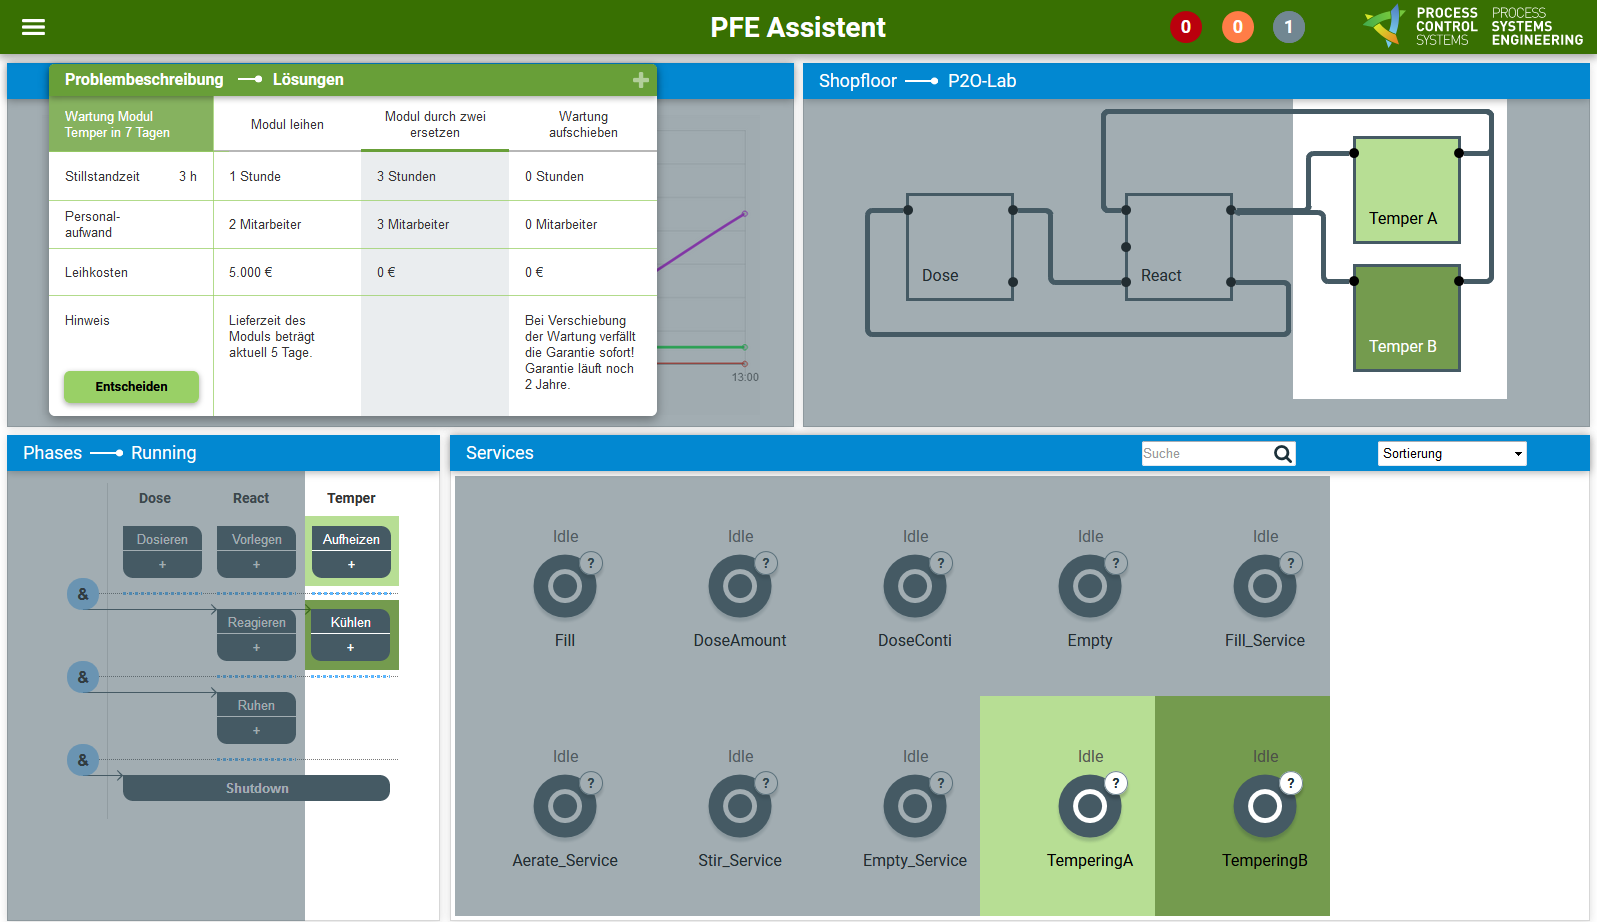
\includegraphics[scale=0.4]{DA_files/Prototyp-PFE-Loesung2.png}
\caption{Darstellung einer Lösung für ein Problem}
\end{figure}

\section{Validierung}
Wie gut / schlecht kam der Entwurf an? Was fehlt noch?

\section{Zusammenfassung}
Nutzer kann mit entsprechenden Informationen geeignet unterstützt werden. Offen bleibt, wie der Nutzer selber Probleme und Lösungen eingeben kann.


 {\tiny\renewcommand{\section}[2]{}%
 	 \begin{thebibliography}{8.5}
 	 \bibitem{bainbridget_ironies_1983}
 	 	Lisanne Bainbridget. {\glqq Ironies of Automation\grqq}. {In: \textit{Automatica}} 19.6 (1983), s. 775-779.
	\end{thebibliography}}
	
\end{document}